% !TeX root = ../../main.tex
\begingroup
\ChSixBegin
\ChFiveBegin
\emergencystretch=2em
% Keep breakable prompt boxes within the fixed CMU text height.
\tcbset{pad at break*/.append style={enlargepage flexible=0pt}}
\appendix{Constructing and Validating Patient Trajectories via Textual Time Series}\label{app:ch05}\label{app:ch06}
This appendix supports the reconstruction studies in Chapter~\ref{chap:ch05}.

% !TeX root = ../../../main.tex

\subsection{Corpora, Reference Annotations, and Model Configurations}\label{ch05:apd:corpora-configurations}

Table~\ref{ch06:tab:dataset-summary} summarizes the evaluation populations and their reference annotations.

Figures~\ref{ch05:fig:record_schema} and~\ref{ch05:fig:demo} show the PMOA-TTS record schema and cohort demographics.

% !TeX root = ../../../../main.tex
\subsubsection{Annotated PMOA Subsets}
\label{ch06:apd:subset_ids}

The \texttt{sepsis-40} subset contains 40 PMOA case reports with manual clinician annotations, yielding $3,229$ reference clinical events.
The \texttt{sepsis-10} subset is a 10-report subset (801 reference events) of \texttt{sepsis-40} used for clinician annotation quality review, hallucination audit, multi-pass self-consistency, and sepsis onset analysis.


% !TeX root = ../../../../main.tex
\begin{table}[htbp]
\caption{
PMCID composition of the annotated PMOA subsets for \texttt{sepsis-40}.\\
A checkmark indicates membership in \texttt{sepsis-10}.
}\ChSixFloatLabel{ch06:tab:subset_pmcs}
\ChSixTableBodyStart
\begin{ChSixFloatBody}

\centering


\begin{tabular}{lc@{\hspace{3em}}lc}
\toprule
PMCID & \texttt{sepsis-10} & PMCID & \texttt{sepsis-10} \\
\midrule
PMC10037274 &  & PMC10493687 &  \\
PMC3075162  & \checkmark & PMC4421677  &  \\
PMC4929359  &  & PMC5862012  &  \\
PMC6345085  &  & PMC7331532  &  \\
PMC8546416  &  & PMC9355071  & \checkmark \\
PMC10370906 & \checkmark & PMC10556716 & \checkmark \\
PMC3130983  &  & PMC4573216  &  \\
PMC5142474  &  & PMC6059163  &  \\
PMC6441647  &  & PMC7451141  &  \\
PMC8855197  &  & PMC9393191  &  \\
PMC10406025 &  & PMC10629858 & \checkmark \\
PMC3325348  &  & PMC4778217  & \checkmark \\
PMC5721301  &  & PMC6231299  &  \\
PMC6910033  &  & PMC7576661  & \checkmark \\
PMC9136437  & \checkmark & PMC9552858  & \checkmark \\
PMC10480000 &  & PMC2698425  &  \\
PMC4120057  &  & PMC4898175  &  \\
PMC5747955  &  & PMC6238558  & \checkmark \\
PMC7093739  &  & PMC8298783  &  \\
PMC9260376  &  & PMC9647393  &  \\
\bottomrule
\end{tabular}

\end{ChSixFloatBody}
\end{table}


\FloatBarrier

% !TeX root = ../../../main.tex
\begin{figure}[htbp]
\begin{ChFiveFloatBody}

\centering

\begin{minipage}[t]{1\textwidth}
\centering
\footnotesize
\begin{adjustbox}{max width=\linewidth}\begin{tabular}{@{} l l >{\raggedright\arraybackslash}p{4cm} @{}}
\toprule
\textbf{Field} & \textbf{Type} & \textbf{Description} \\
\midrule
\texttt{pmc\_id} & str &
Folder-level ID (PMC000xxxxxx--PMC011xxxxxx). \\

\texttt{case\_report\_id} & str &
Filename of the case (e.g., PMC6417290). \\

\texttt{textual\_timeseries} & List[Dict] &
Sequence of \{"event": str, "time": int\}. \\

\texttt{demographics} & Dict &
\{"age": str/"Not Specified", "sex": str, "ethnicity": str\}. \\

\texttt{diagnoses} & List[str] &
List of diagnosis terms extracted per case. \\

\bottomrule
\end{tabular}\end{adjustbox}
\end{minipage}
\hfill

\begin{minipage}[t]{\linewidth}
\centering
\begin{tcolorbox}[
  colback=gray!5,
  colframe=gray!70,
  title=Example JSON entry,
  boxrule=1pt,
  enhanced,
  %breakable,
  fontupper=\footnotesize
]
\begin{verbatim}
"pmc_id": "PMC006xxxxxx",
"case_report_id": "PMC6417290",

"textual_timeseries": [
  {"event": "56 years old", "time": 0},
  {"event": "male", "time": 0},
  {"event": "HIV-positive", "time": 0},
  {"event": "admitted to the hospital", "time": 0},
  {"event": "knee arthralgia", "time": 0},
  ...
  {"event": "postural headache", "time": 48},
  {"event": "neurological examination", "time": 120},
  {"event": "persistence of headache", "time": 144},
  {"event": "brain computed tomography scan",
   "time": 144},
  ...
  {"event": "symptom free", "time": 4320},
  {"event": "CT scan", "time": 4320},
  {"event": "no brain shift", "time": 4320}
],
"diagnoses": [
  "HIV",
  "Knee arthralgia",
  "Subdural hematoma",
  "Postdural puncture headache (PDPH)"
],
"demographics": {
  "age": 56,
  "sex": "Male",
  "ethnicity": "Not Specified"
}
\end{verbatim}
\end{tcolorbox}
\end{minipage}





\end{ChFiveFloatBody}
\caption{\textbf{top:} PMOA-TTS record schema. \textbf{bottom:} compact example matching the schema above (drawn from our HuggingFace repository (formatted for readability).}\ChFiveFloatLabel{ch05:fig:record_schema}
\end{figure}

% !TeX root = ../../../main.tex
\begin{figure}[htbp]
\begin{ChFiveFloatBody}

  \centering
  \begin{minipage}[t]{0.49\linewidth}
    \centering
    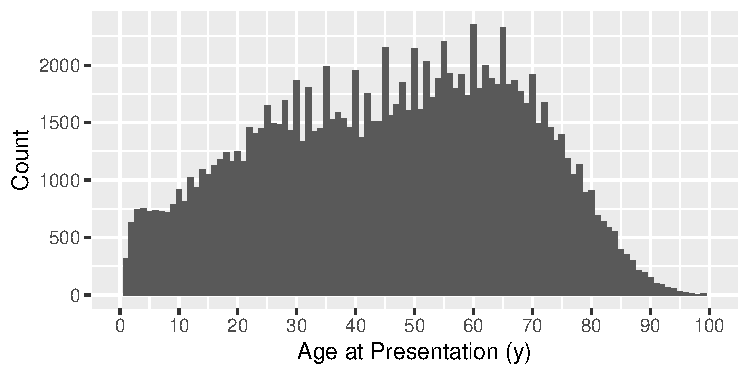
\includegraphics[width=\linewidth]{Appendices/appendix-ch05/images/Scientific_data/Plots_tables/125k_age.pdf}
  \end{minipage}\hfill
  \begin{minipage}[t]{0.49\linewidth}
    \centering
    \scriptsize
    \begin{tabular}{l r}
      \toprule
      \textbf{Characteristic} & \textbf{Percent (\%)}\\
      \midrule
      \multicolumn{2}{l}{\textbf{Sex}}\\
      \quad Male & 52\\
      \quad Female & 47\\
      \quad Not Specified & 1\\
      \midrule
      \multicolumn{2}{l}{\textbf{Ethnicity}}\\
      \quad White/Caucasian & 5\\
      \quad Asian & 3\\
      \quad African & 1\\
      \quad Other & 2\\
      \quad Not Specified & 89\\
      \bottomrule
    \end{tabular}
  \end{minipage}
  
  
  

\end{ChFiveFloatBody}
\caption{\ChFiveRebuttal{Age distribution and LLM-mapped/extracted demographic descriptors for 124{,}349 PMOA-TTS case reports.}}\ChFiveFloatLabel{ch05:fig:demo}
\end{figure}

\FloatBarrier

% !TeX root = ../../../main.tex
\subsubsection{UMLS Mapping for Diagnosis Standardization}
\label{ch05:apd:umls-mapping}

To standardize the diagnoses extracted by LLMs from the case reports, we mapped the free-text diagnoses to concepts in the Unified Medical Language System (UMLS). 
This process involved the following steps:

\begin{enumerate}
    \item \textbf{Initial Extraction}: For each case report, we prompted the LLM to extract diagnoses. 
    This yielded a list of free-text diagnoses for each case report.

    \item \textbf{Entity Linking}: We used ScispaCy's entity linker model 
    \texttt{(en\_core\_sci\_lg)} with the UMLS knowledge base to map each extracted diagnosis to corresponding UMLS Concept Unique Identifiers (CUIs). 
    \ChFiveRebuttal{Each complete extracted diagnosis string is now supplied directly to the UMLS candidate generator.}

    \item \textbf{Filtering and Disambiguation}: For each diagnosis, we:
    \begin{itemize}
        \item Retained only mappings with a confidence score above 0.85.
        \item \ChFiveRebuttal{When candidates are tied or near-tied, the selection procedure favors exact normalized canonical-name matches, recognized canonical suffixes, and concepts whose canonical name contains the complete diagnosis phrase.}
    \end{itemize}

    \item \textbf{Concept Normalization}: After mapping to CUIs, we:
    \begin{itemize}
        \item Retrieved the canonical names from UMLS Metathesaurus.
    \end{itemize}
\end{enumerate}


This mapping process allowed us to standardize the diverse expressions of diagnoses extracted by LLMs into a consistent terminology system, enabling more reliable frequency analysis and co-occurrence patterns. 
Across the full PMOA-TTS corpus, LLM-extracted diagnoses yielded
$N_{\text{raw}} = 63{,}715$ unique free-text diagnosis strings.
Of these, $N_{\text{mapped}} = 41{,}216$ ($64.7\%$) were successfully mapped to at least one
UMLS CUI with a confidence score $\ge 0.85$.
When weighted by frequency of occurrence, mappings at this threshold covered
$91.7\%$ of all diagnosis mentions, indicating that commonly occurring clinical
diagnoses were more likely to receive high-confidence mappings.
Mapping coverage decreased monotonically with increasing confidence threshold.
We therefore selected a threshold of 0.85 as a conservative operating point for
downstream normalization, providing broad coverage of frequently occurring diagnoses
while maintaining a high-confidence mapping criterion.


% !TeX root = ../../../main.tex
\subsubsection{Model and Inference Configuration}
\label{ch05:sec:supp-model-configuration}

Seven large language models were evaluated for textual time series annotation:
Llama 3.3 70B Instruct, DeepSeek-R1, DeepSeek-V3, GPT-5, O4-mini, O3,
and O1.
The exact checkpoint identifiers and Azure deployment names are
reported in Table~\ref{ch05:tab:model-identifiers}.
Llama 3.3 70B Instruct and
DeepSeek-R1 were also used to produce the full-corpus annotations.
Each model
was evaluated across five independent generation runs using the textual time
series prompt in Supplementary Section~\ref{ch05:apd:extraction-prompt}.


Table~\ref{ch05:tab:inference-settings} summarizes the recorded inference
configuration.
Llama 3.3 70B Instruct was run using Hugging Face Transformers
and PyTorch with bfloat16 weights and automatic device placement.
The Azure
OpenAI models were queried through the Chat Completions interface using API
version \texttt{2024-12-01-preview}.
Temperature, top-$p$, and generation seeds
were not explicitly specified for the Azure models.
In all API-based runs, the
complete extraction prompt and case-report text were submitted together as a
single user message, and responses were generated without streaming.


% !TeX root = ../../../main.tex
\begin{table}[htbp]
\caption{
Exact model identifiers and Azure OpenAI deployment names used for textual
time series annotation.
}\ChFiveFloatLabel{ch05:tab:model-identifiers}
\ChFiveTableBodyStart
\begin{ChFiveFloatBody}

\centering


\scriptsize
\setlength{\tabcolsep}{6pt}
\renewcommand{\arraystretch}{1.15}
\begin{tabular}{>{\raggedright\arraybackslash}p{0.31\linewidth} >{\raggedright\arraybackslash}p{0.61\linewidth}}
\toprule
\textbf{Model} &
\textbf{Checkpoint identifier or API deployment} \\
\midrule

Llama 3.3 70B Instruct &
\texttt{meta-llama/Llama-3.3-70B-Instruct} \\

DeepSeek-R1 &
\texttt{deepseek-ai/DeepSeek-R1-0528} \\

DeepSeek-V3 &
\texttt{deepseek-ai/DeepSeek-V3-0324} \\

GPT-5 &
Azure OpenAI deployment \texttt{gpt-5} \\

O4-mini &
Azure OpenAI deployment \texttt{o4-mini} \\

O3 &
Azure OpenAI deployment \texttt{o3} \\

O1 &
Azure OpenAI deployment \texttt{o1} \\

\bottomrule
\end{tabular}

\end{ChFiveFloatBody}
\end{table}



% !TeX root = ../../../main.tex
\begin{table}[htbp]
\caption{
Inference and generation settings used for textual time series annotation.
Parameters described as not explicitly set were not supplied in the
corresponding generation request.
}\ChFiveFloatLabel{ch05:tab:inference-settings}
\ChFiveTableBodyStart
\begin{ChFiveFloatBody}

\centering


\scriptsize
\setlength{\tabcolsep}{5pt}
\renewcommand{\arraystretch}{1.18}
\begin{tabular}{
    >{\raggedright\arraybackslash}p{0.18\textwidth}
    >{\raggedright\arraybackslash}p{0.28\textwidth}
    >{\raggedright\arraybackslash}p{0.47\textwidth}
}
\toprule
\textbf{Model or configuration} &
\textbf{Inference framework and precision} &
\textbf{Generation settings} \\
\midrule

Llama 3.3 70B Instruct
(full-corpus annotation) &
Hugging Face Transformers and PyTorch;
bfloat16;
automatic device placement &
128k-token model context;
batch size 1;
\texttt{max\_new\_tokens=8092};
\texttt{do\_sample=True};
\texttt{top\_k=1};
one returned sequence;
temperature and top-$p$ not explicitly set;
no explicit generation seed \\

Llama 3.3 70B Instruct
(technical validation) &
Hugging Face Transformers and PyTorch;
bfloat16;
automatic device placement &
128k-token model context;
batch size 1;
\texttt{max\_new\_tokens=8092};
\texttt{do\_sample=True};
\texttt{temperature=1};
\texttt{top\_k=1};
one returned sequence;
no explicit generation seed \\

DeepSeek-R1 &
DeepSeek-V3 architecture;
checkpoint configuration specifies bfloat16 with FP8 block quantization &
163{,}840-position context;
five independent generation runs using the production textual time series
prompt \\

DeepSeek-V3 &
DeepSeek-V3 architecture;
checkpoint configuration specifies bfloat16 with FP8 block quantization &
163{,}840-position context;
five independent generation runs using the production textual time series
prompt \\

GPT-5 &
Azure OpenAI Chat Completions;
provider-managed numerical precision &
API version \texttt{2024-12-01-preview};
\texttt{max\_completion\_tokens=16834};
\texttt{stream=False};
temperature, top-$p$, and API seed not explicitly set \\

O4-mini, O3, and O1 &
Azure OpenAI Chat Completions;
provider-managed numerical precision &
API version \texttt{2024-12-01-preview};
\texttt{max\_completion\_tokens=40000};
\texttt{stream=False};
temperature, top-$p$, and API seed not explicitly set \\

\bottomrule
\end{tabular}

\end{ChFiveFloatBody}
\end{table}


\subsubsection{Sepsis Reconstruction Study Configuration}

Table~\ref{ch06:tab:study-configuration} retains the sepsis study configuration, including the phenotype counts and reference models.

% !TeX root = ../../../../main.tex
\begin{table}[htbp]
\caption{Sepsis reconstruction study configuration. Bold cells indicate contributed labeling}\ChSixFloatLabel{ch06:tab:study-configuration}
\ChSixTableBodyStart
\begin{ChSixFloatBody}




\centering
\begin{adjustbox}{width=0.8\textwidth}
\begin{tabular}{|>{\raggedright\arraybackslash}p{3.5cm}|>{\raggedright\arraybackslash}p{3.5cm}|>{\raggedright\arraybackslash}p{3.5cm}|>{\raggedright\arraybackslash}p{3.5cm}|}
\hline
\textbf{Corpus}                  & \centering \textbf{i2m4}             & \centering \textbf{\texttt{sepsis-40}}& \textbf{\qquad \texttt{sepsis-100}}       \\
\hline
\textbf{N (unlabeled)}          & \multicolumn{1}{r|}{310;  331,794}             & \multicolumn{1}{r|}{2,139}                     & \multicolumn{1}{r|}{2,139}                      \\ \hline
\textbf{N (labeled)}            & \multicolumn{1}{r|}{20}                         & \multicolumn{1}{r|}{40}                       & \multicolumn{1}{r|}{100}                       \\ \hline
\textbf{Source}                 & i2b2; MIMIC IV           & PMOA       & PMOA       \\ \hline
\textbf{Note type}              & discharge summary        & case report              & case report               \\ \hline
\textbf{Labeler}                & \textbf{clinicians}               & \textbf{clinicians} (Gold)& \textbf{GPT-5} (Bronze)\\ \hline
\textbf{Phenotyper}             & \textbf{clinicians}      & \textbf{clinicians}      & \textbf{QwQ-32B-Preview}             \\ \hline
\textbf{Methods}                &                & GPT-5& GPT-5\\ 
                                & DeepSeek-R1& DeepSeek-R1& DeepSeek-R1\\ 
                                & L3.3 70B Instruct                  & L3.3 70B Instruct                & L3.3 70B Instruct                 \\ 
                                & L3.1 70B Instruct                 & L3.1 70B Instruct                & L3.1 70B Instruct   \\ 
                                & Mixtral 8x7B & Mixtral 8x7B                & Mixtral 8x7B                   \\ 
                                & \quad Instruct v0.1 & \quad Instruct v0.1                & \quad Instruct v0.1                   \\ 
                                & L3.1 8B Instruct             & L3.1 8B Instruct                & L3.1 8B Instruct                  \\ \hline
\parbox{3cm}{\textbf{Ablations}} & No role                  & No role                  & No role                   \\ 
Base: & No conjunction & No conjunction & No conjunction
                                \\ 
L3.3 70B Instruct                        & \quad instruction &  \quad instruction & \quad instruction \\
                                
                                & No few-shot prompting    & No few-shot prompting    & No few-shot prompting     \\ \hline
\textbf{Sensitivity analyses}   & With upper bound         & With upper bound         & With upper bound          \\ 
                                & With upper bound + 
                                                         & With upper bound +  
                                                                                      & With upper bound + \\
                                & \quad i2b2 event typing & \quad i2b2 event typing & \quad i2b2 event typing \\
                                                                                      \hline
\end{tabular}
\end{adjustbox}

\end{ChSixFloatBody}
\end{table}


\FloatBarrier

% !TeX root = ../../../main.tex
\subsection{Extraction, Provenance, and Clinical Prompts}
\label{ch05:apd:llm-prompts}

\ChFiveHeadingOnly
\subsubsection{LLM Prompt to Generate Textual Time Series from PMOA Case Reports}
\label{ch05:apd:extraction-prompt}

\begin{tcolorbox}[
  colback=gray!5,
  colframe=gray!100,
  title=Prompt,
  boxrule=2pt,
  enhanced,
  breakable,                % <-- allows page breaks; starts here even if long
  before skip=8pt,          % spacing above (optional)
  after skip=8pt,           % spacing below (optional)
  pad at break*=2mm,        % padding at page break (optional)
  fontupper=\scriptsize,
  title after break={Prompt} % optional continuation note
]
You are a physician. Extract the clinical events and the related time stamp from the case report. The admission event has timestamp 0. If the event is not available, we treat the event, e.g. current main clinical diagnosis or treatment with timestamp 0. The events that happened before event with 0 timestamp have negative time, the ones after the event with 0 timestamp have positive time. The timestamp are in hours. The unit will be omitted when output the result. If there is no temporal information of the event, please use your knowledge and events with temporal expression before and after the events to provide an approximation. We want to predict the future events given the events happened in history. For example, here is the case report.\\

\textcolor{teal}{\texttt{An 18-year-old male was admitted to the hospital with a 3-day history of fever and rash. Four weeks ago, he was diagnosed with acne and received the treatment with minocycline, 100 mg daily, for 3 weeks. With increased WBC count, eosinophilia, and systemic involvement, this patient was diagnosed with DRESS syndrome. The fever and rash persisted through admission, and diffuse erythematous or maculopapular eruption with pruritus was present. One day later the patient was discharged.}}\\

Let's find the locations of events in the case report.
The phrase ‘a 3-day history of fever and rash’ directly places fever and rash 72 hours before admission, so both events receive timestamp \(-72\). The phrase ‘Four weeks ago’ directly places the acne diagnosis and initiation of minocycline treatment 672 hours before admission, so both events receive timestamp \(-672\). The diffuse erythematous or maculopapular eruption with pruritus is described in the admission context and is assigned timestamp 0. DRESS syndrome has no explicit timestamp, so clinical judgment is used to assign timestamp 0. The phrase ‘One day later’ places discharge 24 hours after admission.
% it shows that four weeks ago of fever and rash, four weeks ago, he was diagnosed with acne and receive treatment. So the event of fever and rash happened four weeks ago, 672 hours, it is before admitted to the hospital, so the time stamp is -672. diffuse erythematous or maculopapular eruption with pruritus was documented on the admission exam, so the timestamp is 0 hours, since it happens right at admission. DRESS syndrome has no specific time, but it should happen soon after admission to the hospital, so we use our clinical judgment to give the diagnosis of DRESS syndrome the timestamp 0. 
The output should look like:\\

%\vspace{2mm}
\texttt{18 years old | 0 \\
male | 0 \\
admitted to the hospital | 0 \\
fever | -72 \\
rash | -72 \\
acne | -672 \\
minocycline | -672 \\
increased WBC count | 0 \\
eosinophilia| 0 \\
systemic involvement| 0 \\
diffuse erythematous or maculopapular eruption| 0 \\
pruritis | 0 \\
DRESS syndrome | 0 \\
fever persisted | 0 \\
rash persisted | 0 \\
discharged | 24} \\

Separate conjunctive phrases into their component events and assign them the same timestamp (for example, separation of ‘fever and rash’ into 2 events: ‘fever’ and ‘rash’). If the event has duration, assign the event time as the start of the time interval. Attempt to use the text span without modifications except ‘history of’ where applicable. Include all patient events, even if they appear in the discussion; do not omit any events; include termination/discontinuation events; include the pertinent negative findings, like ‘no shortness of breath’ and ‘denies chest pain’. Show the events and timestamps in rows, each row has two columns: one column for the event, the other column for the timestamp. The time is a numeric value in hour unit. The two columns are separated by a pipe ‘|’ as a bar-separated file. Reply with the table only.
\end{tcolorbox}


\subsubsection{LLM Prompt to Extract Demographics from PMOA Case Reports}
\label{ch05:apd:demographics-prompt}

\ChFiveRebuttal{The prompt below is reproduced verbatim for reproducibility. Its outputs are described in the manuscript as LLM-extracted sex descriptors and LLM-mapped ethnicity categories, not as verified biological or self-identified attributes.}

\begin{tcolorbox}[
  colback=gray!5,
  colframe=gray!100,
  title={Prompt},
  boxrule=2pt,
  enhanced,
  breakable,                % <-- allows page breaks; starts here even if long
  before skip=8pt,          % spacing above (optional)
  after skip=8pt,           % spacing below (optional)
  pad at break*=2mm,        % padding at page break (optional)
  fontupper=\scriptsize,
  title after break={{Prompt}} % optional continuation note
]
You are an expert clinician. Extract the following demographic information from the case report: (1) age at case presentation, (2) sex (biologic sex at birth), and (3) ethnicity.  Report the age in years.  Report the sex as Male, Female, otherwise as a custom string, or Not Specified.  Report ethnicity as according to the US Census, otherwise as Not Specified.  For example, here is the case report.\\

\textcolor{teal}{\texttt{An 18-year-old male was admitted to the hospital with a 3-day history of fever and rash. Four weeks ago, he was diagnosed with acne and received the treatment with minocycline, 100 mg daily, for 3 weeks. With increased WBC count, eosinophilia, and systemic involvement, this patient was diagnosed with DRESS syndrome. The fever and rash persisted through admission, and diffuse erythematous or maculopapular eruption with pruritus was present. One day later the patient was discharged.}}\\

% \noindent
Then the demographic extraction should be:\\
\texttt{18 | Male | Not Specified} \\
 
Report the demographics with the three columns separated by a pipe '|' as a bar-separated row as above.
\end{tcolorbox}
\subsubsection{LLM Prompt to Extract List of Diagnoses from PMOA Case Reports}
\label{ch05:apd:diagnosis-prompt}
\begin{tcolorbox}[
  colback=gray!5,
  colframe=gray!100,
  title=LLM prompt to extract list of diagnoses from PMOA case reports,
  boxrule=2pt,
  enhanced,
  breakable,                % <-- allows page breaks; starts here even if long
  before skip=8pt,          % spacing above (optional)
  after skip=8pt,           % spacing below (optional)
  pad at break*=2mm,        % padding at page break (optional)
  fontupper=\scriptsize,
  title after break={Prompt} % optional continuation note
]
\textcolor{teal}{\texttt{An 18-year-old male was admitted to the hospital with a 3-day history of fever and rash. Four weeks ago, he was diagnosed with acne and received the treatment with minocycline, 100 mg daily, for 3 weeks. With increased WBC count, eosinophilia, and systemic involvement, this patient was diagnosed with DRESS syndrome. The fever and rash persisted through admission and diffuse erythematous or maculopapular eruption with pruritus was present. One day later the patient was discharged.}} \\

Then the output should look like:\\
    \texttt{acne} \\
    \texttt{DRESS syndrome} \\

Rash, leukocytosis, and other findings are not diseases so they are omitted, while acne and DRESS syndrome were both diagnosed, so they are included. Output a list of diagnoses (one per line) from the following case. Place the primary diagnosis first. Include only the list and nothing else.

\end{tcolorbox}

\subsubsection{Timestamp Provenance Audit Prompt}
\label{ch05:apd:timestamp-provenance-prompt}
\begin{tcolorbox}[
  colback=gray!5,
  colframe=gray!100,
  title={Prompt},
  boxrule=2pt,
  enhanced,
  breakable,                % <-- allows page breaks; starts here even if long
  before skip=8pt,          % spacing above (optional)
  after skip=8pt,           % spacing below (optional)
  pad at break*=2mm,        % padding at page break (optional)
  fontupper=\scriptsize,
  title after break={{Prompt}} % optional continuation note
]
You are a physician. Extract all patient-specific clinical events and their related timestamps from the case report.


TEMPORAL ANCHOR AND TIMESTAMPS


- Assign timestamp 0 to the hospital admission event when admission is described.

- If an admission event is not available, assign timestamp 0 to the current main clinical presentation, diagnosis, or treatment used as the case reference event.

- Events before the timestamp-0 event have negative timestamps, and events after the timestamp-0 event have positive timestamps.

- Express every timestamp as a numeric value in hours and omit the unit from the output.

- If the report does not provide enough temporal information to determine an event time from the text, use surrounding events, narrative order, and clinical knowledge to provide an approximate timestamp.


KNOWN FLAG: TEXT-SUPPORTED OR RULE-DETERMINED VS \\
MODEL-IMPUTED


Add a third output column named \texttt{known}. The purpose of this flag is to distinguish timestamps that are supported by the report or fixed annotation rules from timestamps that the model has to impute or guess.

Set \texttt{known} to 1 when the assigned timestamp is supported by the source text or is fixed by the annotation rules. This includes any of the following:

- The text gives an absolute date or time, a duration, or a relative temporal expression that can be converted to hours.

- The text explicitly relates the event to the timestamp-0 event, such as ``at admission'', ``on presentation'', ``before admission'', ``after admission'', or ``hospital day 2''.

- The event itself defines the timestamp-0 anchor.

- A temporal expression in the same sentence, clause, list, paragraph, or immediately preceding sentence clearly governs the event, even when the event does not repeat the temporal phrase.

- The event is one of several findings, treatments, or outcomes described as occurring during the same explicitly timed encounter, examination, procedure, or follow-up.

- The timestamp is assigned by a fixed annotation convention rather than model judgment, such as assigning age and sex to timestamp 0.

Set \texttt{known} to 0 only when the source text does not provide enough temporal evidence for the assigned numeric timestamp and the model must supply the time using clinical judgment, an unstated assumption, narrative order alone, interpolation between other events, or another guess.

Important rules for the \texttt{known} flag:

- Do not set \texttt{known} to 0 merely because the event lacks its own temporal phrase. If the event inherits a clear time from the surrounding text, set \texttt{known} to 1.

- Converting an explicit expression such as ``three days before admission'' to -72 hours is \texttt{known = 1}.

- A vague ordering word such as ``later'' or ``subsequently'' supports event order but not a specific number of hours. If a numeric timestamp must be guessed, set \texttt{known} to 0.

- A timestamp of 0 is not automatically known. Set \texttt{known} to 1 only when timestamp 0 is supported by the text, defines the anchor, or follows a fixed annotation convention. Otherwise, set \texttt{known} to 0.

- Use \texttt{known = 0} only for genuinely model-imputed or guessed timestamps.


EXAMPLE CASE REPORT\\


\textcolor{teal}{\texttt{An 18-year-old male was admitted to the hospital with a 3-day history of fever and rash. Four weeks ago, he was diagnosed with acne and received treatment with minocycline, 100 mg daily, for 3 weeks. With increased WBC count, eosinophilia, and systemic involvement, this patient was diagnosed with DRESS syndrome. The fever and rash persisted through admission, and diffuse erythematous or maculopapular eruption with pruritus was present. One day later the patient was discharged.}} \\


EXAMPLE REASONING


The fixed annotation convention assigns age and sex to timestamp 0, so these rows have \texttt{known = 1} because their times are rule-determined rather than guessed. Admission explicitly defines timestamp 0 and has \texttt{known = 1}. The phrase ``a 3-day history of fever and rash'' directly places fever and rash 72 hours before admission, so both events have timestamp -72 and \texttt{known = 1}. The phrase ``Four weeks ago'' directly places the acne diagnosis and start of minocycline treatment 672 hours before admission, so both events have timestamp -672 and \texttt{known = 1}. Increased WBC count, eosinophilia, systemic involvement, and the DRESS syndrome diagnosis have no textual evidence that determines a specific numeric time; assigning them timestamp 0 requires clinical judgment, so they have \texttt{known = 0}. The phrase ``persisted through admission'' explicitly links persistent fever and rash to admission. The diffuse eruption and pruritus are described in the same admission-context sentence, so these events inherit timestamp 0 from that textual context. These events therefore have \texttt{known = 1}. ``One day later'' directly places discharge 24 hours after admission, so discharge has timestamp 24 and \texttt{known = 1}.


EXAMPLE OUTPUT\\


\texttt{18 years old | 0 | 1} \\
\texttt{male | 0 | 1} \\
\texttt{admitted to the hospital | 0 | 1} \\
\texttt{fever | -72 | 1} \\
\texttt{rash | -72 | 1} \\
\texttt{acne | -672 | 1} \\
\texttt{minocycline | -672 | 1} \\
\texttt{increased WBC count | 0 | 0} \\
\texttt{eosinophilia | 0 | 0} \\
\texttt{systemic involvement | 0 | 0} \\
\texttt{diffuse erythematous or maculopapular eruption | 0 | 1} \\
\texttt{pruritus | 0 | 1} \\
\texttt{DRESS syndrome | 0 | 0} \\
\texttt{fever persisted | 0 | 1} \\
\texttt{rash persisted | 0 | 1} \\
\texttt{discharged | 24 | 1} \\


EVENT EXTRACTION RULES


- Separate conjunctive phrases into their component events and assign them the same timestamp. For example, separate ``fever and rash'' into the two events ``fever'' and ``rash''.

- If an event has a duration, assign the event time as the start of the time interval.

- Use the source text span without modification whenever possible, except that ``history of'' may be added where needed to preserve meaning.

- Include all patient-specific events, even when they appear in the discussion.

- Include termination or discontinuation events and pertinent negative findings such as ``no shortness of breath'' and ``denies chest pain''.

- Do not include general medical statements, literature discussion, or events referring to people other than the index patient.


OUTPUT FORMAT


Return one event per row with exactly three pipe-separated columns in this order:\\
\texttt{event | time | known} \\

The time must be numeric and expressed in hours without a unit. The known value must be either 0 or 1. Do not use the pipe character within an event description. Return only the rows. Do not include a header, table title, explanation, Markdown, or code fences.
\end{tcolorbox}

The PMOA-TTS and sepsis reconstruction prompts are reproduced separately to preserve their historical wording.

\begingroup\ChSixBegin

% !TeX root = ../../../../main.tex
\subsubsection{Annotation Prompt}\label{ch06:apd:prompt}
The main annotation prompt used for clinical finding extraction is shown below. 
Specific components are color-coded to relate them directly to the ablation analysis in Section~\ref{ch06:sec:annotation_results_quantitative} and Table~\ref{ch06:tab:sens}: \textcolor{ChSixDarkPurple}{role-playing instruction} (``You are a physician''), \textcolor{ChSixDarkRed}{conjunction expansion}, and \textcolor{ChSixDarkTeal}{few-shot example}.



\begin{tcolorbox}[breakable,
  colback=teal!5,
  colframe=teal!70!black,
  title=Textual Time Series Generation Prompt,
  boxrule=2pt,
]
\footnotesize
\setlength{\parskip}{1pt}
% \singlespacing
\color{ChSixDarkPurple} You are a physician. 

\color{black}  Extract the clinical events and the related time stamp from the case report. The admission event has timestamp 0. If the event is not available, we treat the event, e.g. current main clinical diagnosis or treatment with timestamp 0. The events happened before event with 0 timestamp have negative time, the ones after the event with 0 timestamp have positive time. The timestamp are in hours. The unit will be omitted when output the result. If there is no temporal information of the event, please use your knowledge and events with temporal expression before and after the events to provide an approximation. We want to predict the future events given the events happened in history. 

\color{ChSixDarkTeal} For example, here is the case report.

An 18-year-old male was admitted to the hospital with a 3-day history of fever and rash. Four weeks ago, he was diagnosed with acne and received the treatment with minocycline, 100 mg daily, for 3 weeks. With increased WBC count, eosinophilia, and systemic involvement, this patient was diagnosed with DRESS syndrome. The fever and rash persisted through admission, and diffuse erythematous or maculopapular eruption with pruritus was present. One day later the patient was discharged.

Let's find the locations of event in the case report, it shows that four weeks ago was the acne diagnosis and start of minocycline treatment, four weeks ago, he was diagnosed with acne and receive treatment. So the event of acne diagnosis and start of minocycline treatment happen four weeks ago, 672 hours, it is before admitted to the hospital, so the time stamp is -672. diffuse erythematous or maculopapular eruption with pruritus was documented on the admission exam, so the time stamp is 0 hours, since it happens right at admission. DRESS syndrome has no specific time, but it should happen soon after admission to the hospital, so we use our clinical judgment to give the diagnosis of DRESS syndrome the timestamp 0. Then the output should look like

18 years old $|$ 0\

male $|$ 0\

admitted to the hospital $|$ 0\

fever $|$ -72\

rash $|$ -72\

acne $|$  -672\

minocycline $|$  -672\

increased WBC count $|$ 0\

eosinophilia$|$ 0\

systemic involvement$|$ 0\

diffuse erythematous or maculopapular eruption$|$ 0\

pruritis $|$ 0\

DRESS syndrome $|$ 0\

fever persisted $|$ 0\

rash persisted $|$ 0\

discharged $|$ 24\ 

\color{ChSixDarkRed}
Separate conjunctive phrases into its component events and assign them the same timestamp (for example, the separation of `fever and rash' into 2 events: `fever' and `rash'). 

\color{black} If the event has duration, assign the event time as the start of the time interval. Attempt to use the text span without modifications except `history of' where applicable. Include all patient events, even if they appear in the discussion; do not omit any events; include termination/discontinuation events; include the pertinent negative findings, like `no shortness of breath' and `denies chest pain'.  Show the events and timestamps in rows, each row has two columns: one column for the event, the other column for the timestamp.  The time is a numeric value in hour unit. The two columns are separated by a pipe `$|$' as a bar-separated file. Skip the title of the table. Reply with the table only. Create a table from the following case: 

\textless \textbackslash end prefix\textgreater

\end{tcolorbox}


% !TeX root = ../../../../main.tex
\subsubsection{Phenotyping Prompt}\label{ch06:apd:phenotype-prompt}
For Sepsis-3 determination, we had a clinician review the discharge summaries and assign each case as meeting the Sepsis-3 definition.  
To develop a computational approach, we constructed a prompt specific to Sepsis-3, which describes the qSOFA procedure for determining a Sepsis-3 diagnosis, and used it as query to Llama-3.1-8B-Instruct (L3.1 8B) and QwQ-32B-Preview (Qwen).  
We used the phenotyping prompt:

\begin{tcolorbox}[breakable,
  colback=yellow!10,
  colframe=orange!80!black,
  title=Phenotyping Prompt,
  boxrule=2pt
]
    {You are an expert physician.}  
    
    {Determine if the patient described in the following case report has either sepsis or septic shock, as defined by the Sepsis-3 criteria, which correspond to having a} 
    
    {(1) suspected or confirmed infection and} 
    
    {(2) blood pressure/respiratory rate/mental status abnormalities.} 
    
    {If the information is not present, use your best judgment based on the information available.} 
    
    {Reply 1 for sepsis, 0 otherwise.} 
    
    {Reply with the number 0 or 1 only in \textbackslash\!boxed\{\textbackslash\!n \boxed{<0 $ or $ 1>} \textbackslash\!n\}with no explanation.}
    
    {Here is the case:} 
    
    {\textless \textbackslash end prefix\textgreater}
\end{tcolorbox}


% !TeX root = ../../../../main.tex
\subsubsection{Sepsis onset inference prompt}
\label{ch06:apd:onset_prompt}
We estimate sepsis onset time relative to admission ($t=0$) using a prompt that requests two onset times: one using qSOFA and one using SOFA-style reasoning when sufficient evidence is available.
The model outputs a two-row bar-separated table with onset timestamps in hours (or NA if criteria are not met).

\begin{tcolorbox}[breakable,
  colback=yellow!10,
  colframe=orange!80!black,
  title=Sepsis Onset Prompt,
  boxrule=2pt
]
    You are an astute physician. 
    
    Determine the time of onset of sepsis using two distinct definitions:
    
    (1) using qSOFA, and 
    
    (2) using SOFA, 
    
    relative to the time of admission which has timestamp 0. 
    
    If the admission time is not available, treat the event, e.g. current main clinical diagnosis or treatment with timestamp 0. The events happened before event with 0 timestamp have negative time, the ones after the event with 0 timestamp have positive time. The timestamps are in hours. The unit will be omitted when output the result. 
    
    If there is no temporal information regarding the onset times, please use your knowledge and events with temporal expression before and after the events to provide an approximation. 
    
    Similarly if the numeric quantities in qSOFA/SOFA are not present, use the available text to infer them as needed.
    
    Show the sepsis onsets and timestamps in rows, each row has two columns: one column for the sepsis definition used (qSOFA or SOFA), the other column for the timestamp. 
    
    The time is a numeric value in hour unit. If criteria is not met, set the time to NA. The two columns are separated by a pipe $|$ as a bar-separated file. Skip the title of the table. Create the table from the following case:
    

    {\textless \textbackslash end prefix\textgreater}

\end{tcolorbox}


\endgroup

% !TeX root = ../../../main.tex
\subsection{Event Matching and Reconstruction Metrics}
\label{ch05:apd:evaluation-metrics}

We evaluated textual time series extracted from clinical narratives along three dimensions:
(i) semantic alignment between predicted and manually annotated events (event match recall, precision, and F1),
(ii) agreement in temporal ordering (temporal concordance), and
(iii) agreement in timestamp values (time discrepancy).
Each dimension captures a distinct property of timeline quality.

\subsubsection{Event Match Recall, Precision, and F1}\label{ch05:apd:event-match-rate}\label{ch06:apd:pseudo}

To assess how well predicted clinical events align with reference events, we use a recursive
best-match strategy adapted from prior work~\cite{wang2025large} as shown in Algorithm~\ref{ch05:alg:recursive_match}.
At each step, the method
identifies the closest unmatched pair of predicted and reference events using a text-similarity
metric, retains the pair if it satisfies a distance threshold, and removes both events before
proceeding. \textbf{Algorithm \ref{ch05:alg:recursive_match}} provides pseudocode for this recursive matching procedure.
This strategy produces a one-to-one alignment between reference and predicted events that is
efficient and well-suited to timelines of differing lengths. 

For each list, we use the text order, \emph{i.e.}, the order of the events in the annotation files, to break embedding distance ties.
We use the cosine distance for the distance calculation using sentence transformer embeddings from \texttt{S-PubMedBert-MS-MARCO}.

We evaluated several similarity measures—including Levenshtein distance, BERT-based
embeddings, and PubMedBERT embeddings—and found cosine similarity using PubMedBERT
sentence embeddings to perform best. A cosine distance threshold of 0.1 is used to determine
whether a predicted event is considered a semantic match.

\ChFiveRebuttal{
We evaluate event identification using event match recall, precision, and F1. Let $M$ denote the number of one-to-one semantic matches after assignment and application of the cosine-distance threshold, $N_{\mathrm{ref}}$ the number of reference events, and $N_{\mathrm{model}}$ the number of model-generated events. Event match recall is defined as $M/N_{\mathrm{ref}}$, event match precision as $M/N_{\mathrm{model}}$, and event match F1 as the harmonic mean of precision and recall. Precision therefore penalizes additional model-generated events that remain unmatched under the one-to-one alignment, complementing recall, which measures the proportion of reference events recovered.
}

% !TeX root = ../../../main.tex
\begin{ChFiveAlgorithm}[ht]
\caption{Recursive Best Match}
\scriptsize
\label{ch05:alg:recursive_match}
\begin{algorithmic}[1]
\ChFiveAlgRequire Two lists: \texttt{ref} (manually annotated reference events) and \texttt{pred} (predicted events)
\ChFiveAlgEnsure List of best-matching event pairs
\ChFiveAlgFunction{MatchEvents}{\texttt{ref}, \texttt{pred}}
    \ChFiveAlgIf{\texttt{ref} is empty \textbf{or} \texttt{pred} is empty}
        \ChFiveAlgState \ChFiveAlgReturn \texttt{[]}
    \ChFiveAlgEndIf
    \ChFiveAlgState $\texttt{min\_distance} \gets \infty$
    \ChFiveAlgState $\texttt{best\_pair} \gets \texttt{None}$
    \ChFiveAlgForAll{$r \in \texttt{ref}$}
        \ChFiveAlgForAll{$p \in \texttt{pred}$}
            \ChFiveAlgState $d \gets \texttt{ComputeDistance}(r, p)$
            \ChFiveAlgIf{$d < \texttt{min\_distance}$}
                \ChFiveAlgState $\texttt{min\_distance} \gets d$
                \ChFiveAlgState $\texttt{best\_pair} \gets (r, p)$
            \ChFiveAlgElsIf{$d = \texttt{min\_distance}$}
                \ChFiveAlgState $(r^*, p^*) \gets \texttt{best\_pair}$
                \ChFiveAlgState Get indices (within the annotation files) of $r$, $p$, and also of $r^*, p^*$
                \ChFiveAlgIf{index of $r <$ index of $r^*$}
                    \ChFiveAlgState $\texttt{best\_pair} \gets (r, p)$
                \ChFiveAlgElsIf{index of $r = $ index of $r^*$ \textbf{and} index of $p <$ index of $p^*$}
                    \ChFiveAlgState $\texttt{best\_pair} \gets (r, p)$
                \ChFiveAlgEndIf
            \ChFiveAlgEndIf
        \ChFiveAlgEndFor
    \ChFiveAlgEndFor
    \ChFiveAlgState $(r^*,p^*) \gets \texttt{best\_pair}$
    \ChFiveAlgState Remove $r^*$ from \texttt{ref}
    \ChFiveAlgState Remove $p^*$ from \texttt{pred}
    \ChFiveAlgState $\texttt{result} \gets \texttt{[best\_pair]} + \texttt{MatchEvents}(\texttt{ref}, \texttt{pred})$
    \ChFiveAlgState \ChFiveAlgReturn $\texttt{result}$
\ChFiveAlgEndFunction
\end{algorithmic}
\end{ChFiveAlgorithm}

Algorithm~\ref{ch05:alg:recursive_match} produces the one-to-one pair assignment; applying the cosine-distance threshold of 0.1 to those assigned pairs determines which pairs are accepted as semantic matches.

Recursive matching is the primary method; LAPJV is evaluated as a sensitivity analysis in Appendix~\ref{ch05:apd:lapjv-matching}.

\subsubsection{Temporal Concordance}
\label{ch05:apd:temporal-concordance}

Temporal ordering accuracy is quantified using the concordance index (c-index), which
measures agreement in the ordering of pairs of matched events.
Let $t^{\text{ref}}_i$ and $t^{\text{pred}}_i$ denote the reference and predicted timestamps for
matched event $i$.

\ChFiveRebuttal{
Comparable pairs are formed within each report from matched events with usable timestamps. Pairs with equal reference timestamps are excluded from the concordance denominator. Among the remaining pairs, equal model timestamps receive 0.5 credit. We report the summed number of comparable pairs, the number and percentage of reference ties among all eligible pairs, and the number and percentage of model ties among comparable pairs for each model.
}

The c-index is:
\[
\text{c-index}
=
\frac{1}{N}
\sum_{\substack{i<j\\
t^{\text{ref}}_i \neq t^{\text{ref}}_j}}
\left[
\mathds{1}\!\left\{
(t^{\text{ref}}_i-t^{\text{ref}}_j)
(t^{\text{pred}}_i-t^{\text{pred}}_j)>0
\right\}
+
\frac{1}{2}
\mathds{1}\!\left\{
t^{\text{pred}}_i=t^{\text{pred}}_j
\right\}
\right],
\]
where $N$ is the number of comparable pairs.
Higher values indicate stronger preservation of reference ordering.

\ChFiveRebuttal{
In our analysis of 200 manually annotated benchmark, manual-reference ties accounted for 13.81\%--15.37\% of all eligible pairs, while LLM annotation ties occurred in 14.16\%--34.70\% of comparable pairs (Table \ref{ch05:tab:concordance_pairs_ties}). Counts were summed across documents, and percentages were calculated from the corresponding summed counts. Manual-reference tie rates differ across models because each model yields a different set of matched events with usable timestamps.
}


% !TeX root = ../../../main.tex
\begin{table}[htbp]
\caption{\ChFiveRebuttal{Comparable event pairs and timestamp ties used in the concordance analysis. Manual-reference tie percentages are calculated among all eligible pairs, whereas model tie percentages are calculated among comparable pairs.}}\ChFiveFloatLabel{ch05:tab:concordance_pairs_ties}
\ChFiveTableBodyStart
\begin{ChFiveFloatBody}

\centering
\footnotesize
\setlength{\tabcolsep}{5pt}


\begin{tabular}{lrrr}
\hline
\textbf{Model} &
\textbf{Comparable pairs} &
\begin{tabular}{c}\textbf{Manual-reference}\\\textbf{ties, n (\%)}\end{tabular} &
\begin{tabular}{c}\textbf{Model ties among}\\\textbf{comparable pairs, n (\%)}\end{tabular} \\
\hline
\texttt{Llama 3.3 70B} & 167,738 & 30,470 (15.37\%) & 42,299 (25.22\%) \\
\texttt{DeepSeek-R1}    & 200,183 & 33,937 (14.50\%) & 68,455 (34.20\%) \\
\texttt{DeepSeek-V3}    & 229,576 & 38,338 (14.31\%) & 79,667 (34.70\%) \\
\texttt{OpenAI GPT-5}   & 278,804 & 44,816 (13.85\%) & 39,475 (14.16\%) \\
\texttt{OpenAI O4-mini} & 214,768 & 34,752 (13.93\%) & 56,536 (26.32\%) \\
\texttt{OpenAI O3}      & 203,830 & 32,671 (13.81\%) & 33,255 (16.32\%) \\
\texttt{OpenAI O1}      & 150,708 & 27,190 (15.28\%) & 29,424 (19.52\%) \\
\hline
\end{tabular}

\end{ChFiveFloatBody}
\end{table}

\subsubsection{Time Discrepancy and AULTC}
\label{ch05:apd:aultc}\label{ch06:apd:ltcdf}

For each matched event, we measure timestamp accuracy using the absolute time error.
Because timestamp discrepancies can vary across several orders of magnitude, we evaluate errors on a log scale:
\[
\Delta t_i=|t_i^{\mathrm{pred}}-t_i^{\mathrm{ref}}|,
\qquad x_i=\log(1+\Delta t_i).
\]
We compute the empirical cumulative distribution function
\[
F(x)=\frac{1}{k}\sum_{i=1}^{k}\mathbf{1}\{x_i\leq x\},
\]
where $k$ is the number of semantically matched event pairs in the evaluation.
In the PMOA-TTS evaluation, the empirical CDF is constructed over log-time discrepancies pooled across all matched events in the 200-case reference set.
AULTC is computed over semantically matched event pairs only and therefore measures timestamp accuracy conditional on successful event alignment.
Unmatched events do not enter the empirical CDF or AULTC and are evaluated separately by the event-extraction metrics.
A single common $S_{\max}$ is used to normalize AULTC for all models and runs, avoiding model-specific rescaling.

We compute the AULTC as the area under $F(x)$ from $x=0$ to $x=\log(1+S_{\max})$, normalized by $\log(1+S_{\max})$:
\[
\mathrm{AULTC}
=
\frac{\displaystyle\int_0^{\log(1+S_{\max})}F(x)\,dx}
{\log(1+S_{\max})}.
\]
With this definition, AULTC = 1 indicates that discrepancies are zero (perfect recovery), resulting in maximum area $\log(1+S_{\max})$, and AULTC = 0 indicates that all discrepancies are at or beyond $S_{\max}$, yielding zero area.

\begin{ChSixRemark}
The time unit and cutoff $S_\text{max}$ affect the AULTC calculation, so they must be specified when reporting the AULTC.
\end{ChSixRemark}
Unless otherwise stated, we set $S_{\max}=8760$ hours, corresponding to one year.
This upper limit was chosen because it captures clinically meaningful discrepancies from hours to months while preventing very long-horizon case-history events from dominating the metric.

Because of the $\log(1 + \cdot)$ transformation (rather than the $\log(\cdot)$ transformation which is undefined for zero time-error discrepancy), the discrepancies are non-linearly shifted in the log scale.
The non-linear shift adjusts the relative widths of the step function (particularly for small discrepancies) changing the area calculation.
The cutoff $S_\text{max}$ affects the normalization factor.
Therefore, these values should be chosen based on practicalities for the application.
In our case, we chose hours at the time unit because the only sub-hour descriptions reported were several Apgar scores at the minute-level.

Finally, we stratify timestamp errors by temporal distance (e.g., within 1 hour, 1 day, 1 week,
1 year) to examine how accuracy varies across clinically meaningful time scales.

% !TeX root = ../../../main.tex
\subsection{Uncertainty and Sensitivity Analyses}
\label{ch05:apd:sensitivity-analyses}

\ChFiveHeadingOnly

\subsubsection{Uncertainty Estimates}

Tables~\ref{ch05:tab:bootstrap_intervals} and~\ref{ch06:tab:bootstrap_ci} report case-level bootstrap confidence intervals with the corresponding main results; the across-run standard deviations in Table~\ref{ch05:tab:model_comparison} reflect variation across model generations.

\subsubsection{PMOA-TTS Event-Matching Threshold}

We conducted sensitivity analyses to assess robustness with respect to the event match threshold.
As expected, stricter thresholds produce fewer but cleaner matches, while more permissive thresholds increase coverage at the expense of noisier ordering and timing.
Varying the cosine distance threshold from \ChFiveRebuttal{0.01 to 0.50 (in increments of 0.01 for both the recursive and LAPJV matching analyses)}, we observed corresponding shifts in event match recall, concordance, and AULTC.
A threshold of 0.10 was chosen based on manual review of \texttt{Llama 3.3 70B Instruct} and \texttt{O1} outputs.
The resulting trade-offs are summarized in Figure~\ref{ch05:fig:threshold_tradeoff_greedy}.

\ChFiveRebuttal{For Figure~\ref{ch05:fig:threshold_tradeoff_greedy}, model trajectories change smoothly in the neighborhood of 0.1, but the rank
order is not invariant across the full threshold range, particularly for AULTC where several curves are close or cross.
We therefore interpret the curves as coverage-versus-temporal-accuracy trade-offs rather than evidence of one
threshold-independent winner.}

% !TeX root = ../../../main.tex
\begin{figure}[htbp]
\begin{ChFiveFloatBody}
\centering
        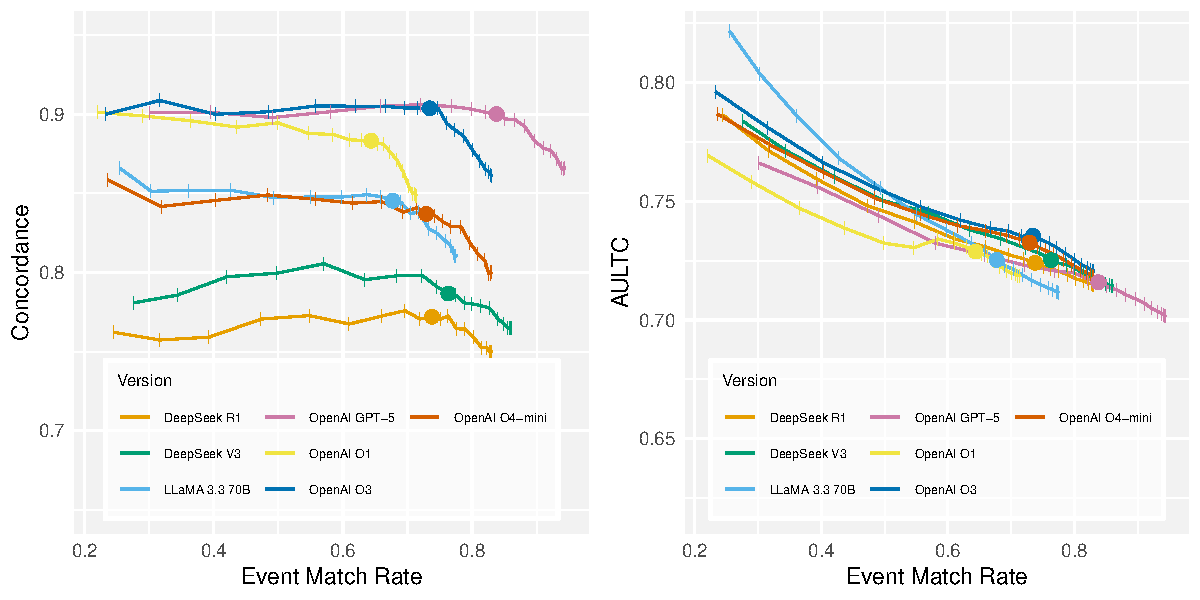
\includegraphics[width=\linewidth]{Appendices/appendix-ch05/images/Scientific_data/Plots_tables/event_match_vs_metrics_updated.pdf}

    
    
    

\end{ChFiveFloatBody}
\caption{Concordance and AULTC by event match rate for recursive matching heuristic. Solid circle ($\bullet$) represents threshold of 0.1, with ticks (|) indicating 0.01 increments of the threshold in [0.01, 0.50].
    }\ChFiveFloatLabel{ch05:fig:threshold_tradeoff_greedy}
\end{figure}

% !TeX root = ../../../../main.tex
\subsubsection{Sepsis Event-Matching Threshold Sensitivity}
\label{ch06:apd:threshold_sweep}

Event matching is performed using cosine distance between PubMedBERT embeddings with threshold $\theta = 0.10$ (Section~\ref{ch06:sec:evaluation_methodology_metrics}).
Because the event match recall depends directly on $\theta$, we conducted a sensitivity analysis by sweeping $\theta$ from $0.01$ to $0.50$ in increments of $0.01$ and recomputing event match recall, concordance, and AULTC for each model.


% !TeX root = ../../../../main.tex
\begin{figure}[htbp]
\begin{ChSixFloatBody}

    \centering
    \begin{minipage}[t]{0.48\columnwidth}
        \centering
        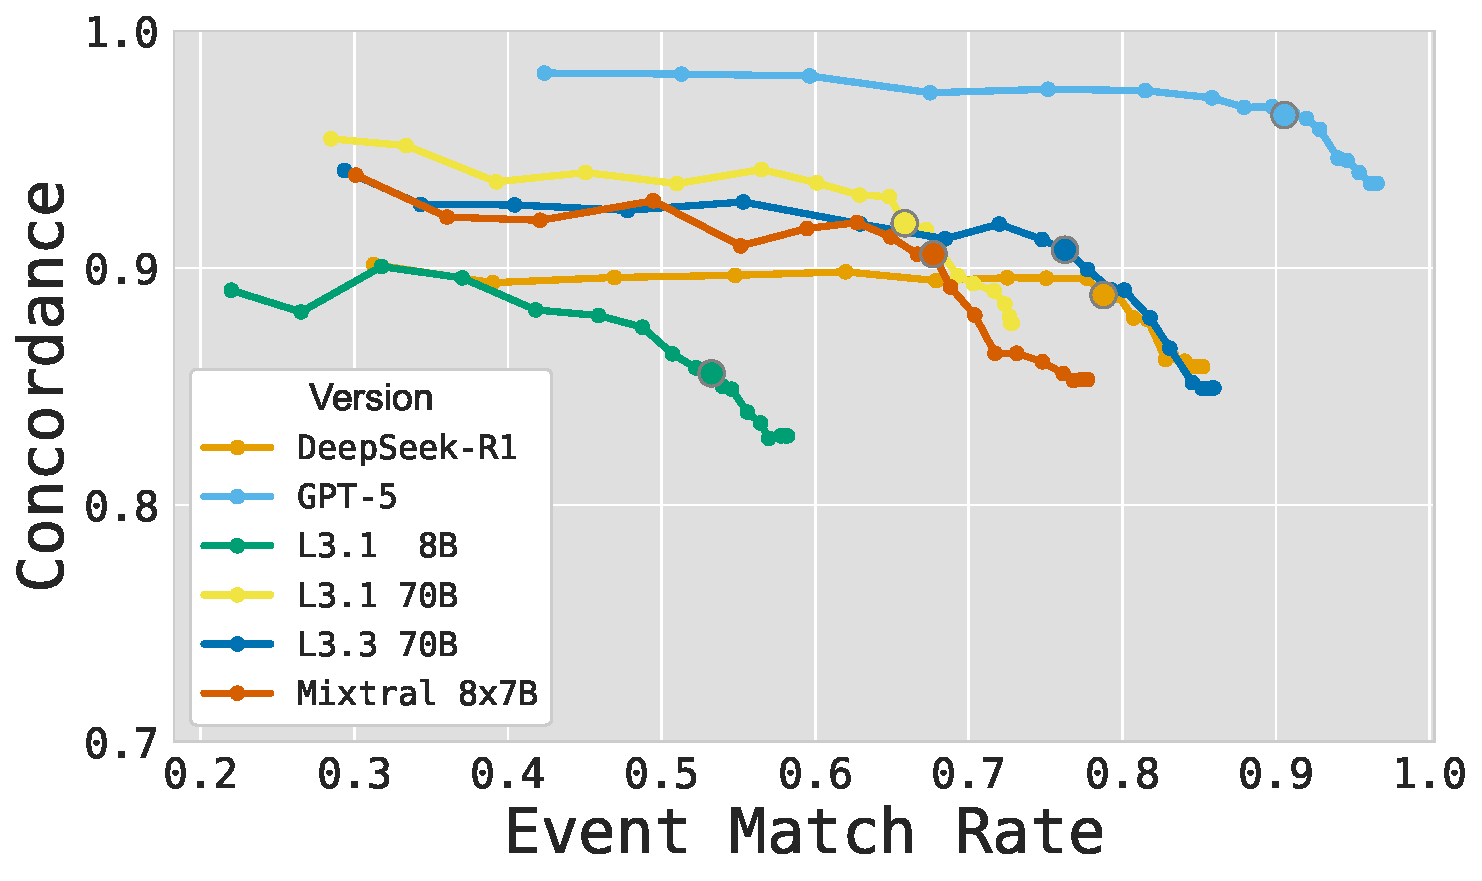
\includegraphics[width=\linewidth]{Appendices/appendix-ch05/sepsis/images/figures/apd_figs/concordance_vs_event_match_rate.pdf}
        
    \end{minipage}\hfill
    \begin{minipage}[t]{0.48\columnwidth}
        \centering
        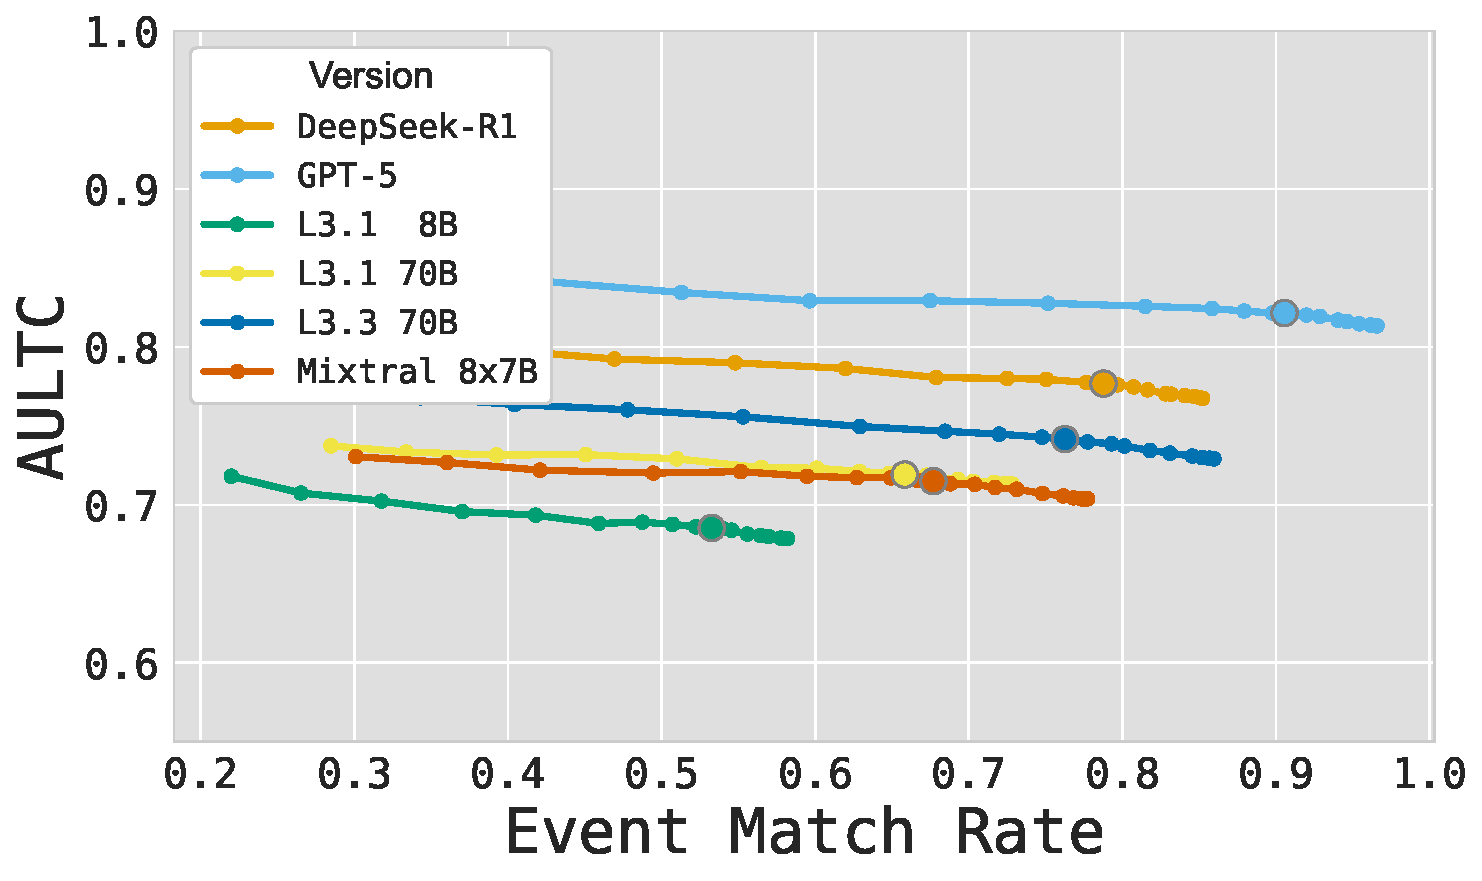
\includegraphics[width=\linewidth]{Appendices/appendix-ch05/sepsis/images/figures/apd_figs/aultc_vs_event_match_rate.pdf}
    \end{minipage}
    
    

\end{ChSixFloatBody}
\caption{Sensitivity of temporal metrics to the cosine distance threshold $\theta$ for the recursive matching heuristic. Left: Concordance versus event match rate obtained by sweeping $\theta$ in increments of $0.01$ over $[0.01, 0.50]$. Right: AULTC versus event match rate under the same sweep. Each point ($\cdot$) corresponds to a distinct threshold value; the solid large circle ($\bullet$) denotes the threshold $\theta = 0.10$ used throughout the paper.}\ChSixFloatLabel{ch06:fig:threshold_sweep}
\ChSixUncaptionedPanelLabel{ch06:fig:threshold_sweep:concordance}
\ChSixUncaptionedPanelLabel{ch06:fig:threshold_sweep:aultc}
\end{figure}


Figure~\ref{ch06:fig:threshold_sweep} shows concordance and AULTC as functions of event match recall induced by varying $\theta$ on the \texttt{sepsis-40} dataset.
As expected, increasing $\theta$ monotonically increases event match recall.
However, beyond a moderate threshold, additional matches correspond to increasingly loose semantic alignments, which degrade temporal metrics.
This produces a characteristic trade-off curve: initial increases in event match recall are accompanied by minimal degradation in concordance and AULTC, followed by a sharper decline once lower-quality matches are admitted.

Across models, we observe a clear ``elbow'' region near $\theta = 0.10$--$0.15$, where event match recall increases modestly while concordance and AULTC remain stable. Beyond this region, particularly past $\theta \approx 0.20$, both concordance and AULTC begin to decline (with concordance drop being more rapid), indicating that additional matches are likely false positive alignments that impair temporal fidelity.

The threshold $\theta = 0.10$ used in the main analysis lies within this elbow region, balancing semantic precision and temporal robustness.
Importantly, relative model ordering remains stable across a wide range of thresholds, suggesting that conclusions regarding comparative performance are not artifacts of a particular cosine distance cutoff of the embeddings.
These results support the use of $\theta = 0.10$ as a conservative and temporally faithful operating point for event matching.





\FloatBarrier


\subsubsection{PMOA-TTS Prompt Sensitivity}
\label{ch05:apd:sensitivity-llm-prompt}

We slightly modified the prompt in Section~\ref{ch05:apd:extraction-prompt} to check for sensitivity to specific parts of the LLM prompt being removed or modified.
This led to the following variants:
\begin{enumerate}\raggedright
    \item \textbf{No changes}: Original LLM query prompt. %
    
    \item \textbf{No role:} Remove the initial sentence \texttt{"You are a physician."}
    
    \item \textbf{Zero-shot prompting:} Remove the example case report and textual time series from the prompt. \\
    \textcolor{teal}{\texttt{An 18-year-old male was admitted to ...}}\\
    "Let's find the locations of events in the case report, it shows that ... then the output should look like:"\\
    \texttt{18 years old | 0 \\
    male | 0 \\
    ..}

    \item \textbf{No conjunction expansion:} Remove the following sentence from the prompt: \texttt{"Separate conjunctive phrases into their component events and assign them the same timestamp (for example, separation of ‘fever and rash’ into 2 events: ‘fever’ and ‘rash’)"}
    
    \item \textbf{Interval:} A query was added to the prompt for extracting the time interval (start and end time of clinical events).
The original prompt’s instructions and few-shot examples were modified accordingly. 
    
    \item \textbf{Interval + Type:} A query was added to the prompt for extracting the time interval and i2b2
    event type (Interval+Type), where event type is one of: Factual, Possible, Hypothetical, Conditional, Negated, Historical, Uncertain.
The original prompt’s instructions and few-shot examples were modified accordingly. 
\end{enumerate}


\ChFiveParagraph{Semantic similarity:}
The cumulative distributions of cosine distances between predicted and reference event phrases show clear differences across prompt variants. \emph{Interval} and \emph{Interval+Type} produce the closest matches, while \emph{Zero-shot} performs substantially worse, with a right-shifted distribution indicating lower-quality event spans. \emph{No role} and \emph{No conjunction} show modest degradation relative to the full prompt.
These results
demonstrate that including structured temporal guidance and explicit event formatting improves semantic alignment.

\ChFiveParagraph{Temporal ordering.}
The concordance index (c-index) follows a similar pattern. \emph{Interval+Type} achieves the highest median concordance, followed by \emph{Interval} and the full prompt.
Removing role
framing or conjunction splitting reduces ordering consistency, and \emph{Zero-shot} again yields the lowest performance with greater variability.
This suggests that structured instructions help the model maintain coherent temporal ordering among extracted events.

\ChFiveParagraph{Timestamp accuracy.}
Overall log-time discrepancy curves show that \emph{Interval} and \emph{Interval+Type} provide the most accurate timestamp predictions, whereas \emph{Zero-shot} exhibits the largest errors.
When stratified by temporal distance from presentation, prompt differences are minimal for
immediate events but widen substantially at longer horizons (1~day, 1~week, 1~year, and beyond).
Structured prompts with explicit temporal cues maintain accuracy across these
intervals, while unstructured prompts degrade more quickly.

When stratified by the time from presentation (e.g., within 1 hour, 1 day, 1 week), prompt differences are most pronounced for events occurring farther from the report anchor (Figure \ref{ch05:fig:prompt_ablation}, far right).
For immediate events, all prompt versions perform comparably.
However, at longer timescales (1 week to "ever"), Interval and Interval+Type maintain superior accuracy, while Zero-shot shows dramatic drops in performance.
This suggests that structured prompts are particularly critical for accurate long-range temporal reasoning.

Across semantic similarity, temporal ordering, and timestamp alignment, prompt components that provide explicit temporal structure or event-typing requirements consistently improve
performance, while removing instructional scaffolding—particularly in the Zero-shot condition—results in substantial degradation.
These findings highlight the importance of prompt
design in guiding LLMs to produce high-quality temporal annotations from clinical narratives.

% !TeX root = ../../../main.tex
\begin{figure}[htbp]
\begin{ChFiveFloatBody}

\centering
    \begin{minipage}[t]{0.242\textwidth}
    \centering
    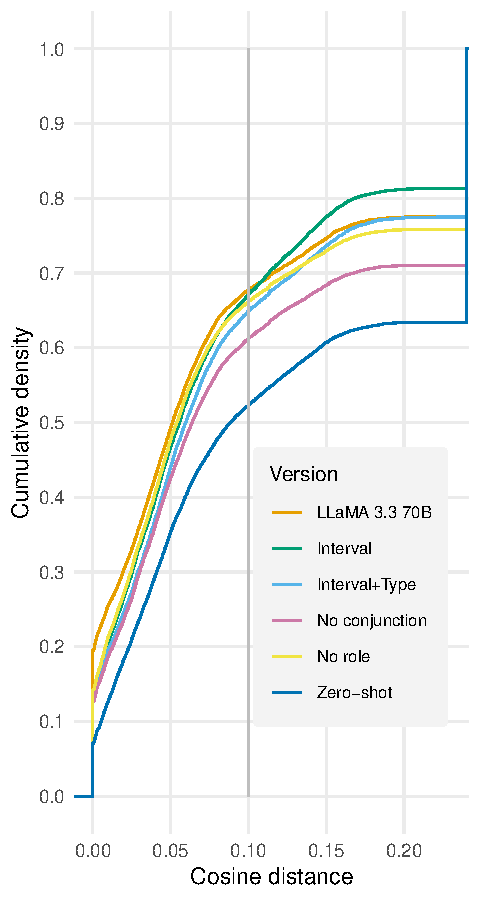
\includegraphics[page=1, width=\linewidth]{Appendices/appendix-ch05/images/Plots_tables/prompt_ablation_updated_figure.pdf}
    \end{minipage}
    \hfill
    \begin{minipage}[t]{0.242\textwidth}
    \centering
    \includegraphics[page=2, width=\linewidth]{Appendices/appendix-ch05/images/Plots_tables/prompt_ablation_updated_figure.pdf}
    \end{minipage}
    \hfill
    \begin{minipage}[t]{0.242\textwidth}
    \centering
    \includegraphics[page=3, width=\linewidth]{Appendices/appendix-ch05/images/Plots_tables/prompt_ablation_updated_figure.pdf}
    \end{minipage}
    \hfill
    \begin{minipage}[t]{0.242\textwidth}
    \centering
    \includegraphics[page=4, width=\linewidth]{Appendices/appendix-ch05/images/Plots_tables/prompt_ablation_updated_figure.pdf}
    \end{minipage}
    
    
    

\end{ChFiveFloatBody}
\caption{Comparison of \texttt{Llama 3.3 70B} prompt ablation and variant methods for extracting temporal clinical events from case reports. From left to right: (\textbf{A}) event match cumulative distribution function, (\textbf{B}) concordance box plots, (\textbf{C}) time discrepancy from manual annotation timestamps among matched events (overall), and (\textbf{D}) time discrepancy disaggregated by clinician annotator timestamp (time from presentation).}\ChFiveFloatLabel{ch05:fig:prompt_ablation}
\end{figure}

\subsubsection{Sensitivity to Event Matching Strategy (LAPJV)}
\label{ch05:apd:lapjv-matching}
We additionally consider a globally optimal one-to-one event alignment based on the Linear Assignment Problem, solved using the Jonker--Volgenant (LAPJV) algorithm \citep{jonker1987shortest}.
We define a rectangular cost matrix whose entries are pairwise cosine distances between predicted and reference events.
To enforce the same distance thresholding used in the recursive heuristic, we assign a large penalty cost to pairs whose distance exceeds the threshold, effectively masking infeasible matches.
LAPJV then computes a minimum-cost assignment under these constraints, yielding a globally optimal one-to-one alignment between the two event sets.

To assess sensitivity to the event alignment procedure, we repeat the inter-LLM comparison using LAPJV-based matching at a cosine distance threshold of 0.1.
Table~\ref{ch05:tab:model_comparison_lapjv} reports event match recall, temporal concordance, and AULTC across five independent runs per model, and is directly comparable to the main-text results obtained using the recursive matching heuristic (Algorithm~\ref{ch05:alg:recursive_match}; Table~\ref{ch05:tab:model_comparison}).

% !TeX root = ../../../main.tex
\begin{table}[htbp]
\caption{\ChFiveRebuttal{Inter-LLM comparison under LAPJV-based event matching (threshold = 0.1), evaluated on 200 manually annotated case reports across five runs per model.}}\ChFiveFloatLabel{ch05:tab:model_comparison_lapjv}
\ChFiveTableBodyStart
\begin{ChFiveFloatBody}


\footnotesize
\centering
\setlength{\tabcolsep}{3pt}


\begin{tabular}{lccccc}
\hline
\textbf{Model} &
\begin{tabular}{c}\textbf{Event Match}\\\textbf{Recall}\end{tabular} &
\begin{tabular}{c}\textbf{Event Match}\\\textbf{Precision}\end{tabular} &
\begin{tabular}{c}\textbf{Event Match}\\\textbf{F1}\end{tabular} &
\textbf{Concordance} &
\textbf{AULTC} \\
\hline
\texttt{Llama 3.3 70B}
& 0.676 $\pm$ 0.003
& 0.761 $\pm$ 0.036
& 0.715 $\pm$ 0.015
& 0.848 $\pm$ 0.003
& 0.720 $\pm$ 0.001 \\

\texttt{DeepSeek-R1}
& 0.750 $\pm$ 0.008
& 0.793 $\pm$ 0.006
& 0.771 $\pm$ 0.006
& 0.773 $\pm$ 0.007
& 0.727 $\pm$ 0.004 \\

\texttt{DeepSeek-V3}
& 0.764 $\pm$ 0.005
& 0.801 $\pm$ 0.005
& 0.782 $\pm$ 0.004
& 0.777 $\pm$ 0.009
& 0.730 $\pm$ 0.002 \\

\texttt{OpenAI GPT-5}
& \textbf{0.851 $\pm$ 0.006}
& 0.761 $\pm$ 0.007
& \textbf{0.803 $\pm$ 0.003}
& \textbf{0.903 $\pm$ 0.004}
& 0.722 $\pm$ 0.001 \\

\texttt{OpenAI O4-mini}
& 0.752 $\pm$ 0.019
& 0.818 $\pm$ 0.015
& 0.783 $\pm$ 0.017
& 0.845 $\pm$ 0.006
& \textbf{0.750 $\pm$ 0.002} \\

\texttt{OpenAI O3}
& 0.738 $\pm$ 0.003
& 0.842 $\pm$ 0.002
& 0.786 $\pm$ 0.002
& 0.900 $\pm$ 0.005
& 0.737 $\pm$ 0.003 \\

\texttt{OpenAI O1}
& 0.640 $\pm$ 0.007
& \textbf{0.878 $\pm$ 0.003}
& 0.740 $\pm$ 0.005
& 0.881 $\pm$ 0.003
& 0.731 $\pm$ 0.002 \\
\hline
\end{tabular}


\end{ChFiveFloatBody}
\end{table}

The additional LAPJV threshold-sweep is available in \citep[Sensitivity Analyses: Sensitivity to Event Matching Strategy (LAPJV)]{noroozizadeh-pmoa-tts-v4}.

% !TeX root = ../../../main.tex

\subsection{Clinical Review, Grounding, and Consistency}\label{ch05:apd:clinical-validation}

These analyses distinguish clinician review, agreement with individual clinicians, factual grounding, generation stability, and agreement between model annotations.

% !TeX root = ../../../main.tex
\subsubsection{Clinician Annotation Quality Review}
\label{ch06:apd:clinician_quality_review}

\ChSixHeadingOnly
\paragraph{Review protocol}

In addition to the quantitative metrics used in the main evaluation, a physician reviewed extracted timelines for the \texttt{sepsis-10} subset.
For each case report, the clinician assigned: (i) a rank ordering (1 = best, 7 = worst) of the annotations, consisting of the manual annotation and six LLM-generated annotations, and (ii) a categorical assessment (Excellent, Good, Acceptable, or Poor) based on extraction completeness, temporal ordering accuracy, and timing plausibility.
This review provides a qualitative assessment of annotation style and clinical usability, complementing the quantitative event-matching and temporal-alignment metrics reported in the main text.
The reviewed annotation bundle included O1-preview as the OpenAI annotation; replacing GPT-5 which was evaluated separately in the main quantitative results in Table~\ref{ch06:tab:results}.

The clinician review results are reported in Table~\ref{ch06:tab:sep10review}.

\ChSixParagraph{Events requiring temporal reasoning or composition.}
Example: ``passed away'' from ``he was re-admitted to the medical ICU for severe sepsis and multiorgan failure and passed away around 6 months after his initial diagnosis with NHL, despite maintaining a remission status.''
This requires a two-step inference: (1) timing of NHL diagnosis, and (2) adding ``around 6 months'' to that time.
While this is a simple example, more complicated chains of relative timing were noted, sometimes involving other events whose timings are themselves uncertain.
As black-box methods, there is no explicit probabilistic specification for these chains, and empirically we see variable responses.
For this case, the manual annotation is 4383 hours (about 6 months), O1-preview gives 4368 hours (about 6 months), DeepSeek-R1 gives 4032 hours (about 6 months), and Llama 3.3 70B gives 1440 hours (about 2 months); compared to other events the temporal ordering is correct, but the relative timing is off by months.


\subsubsection{Model--Clinician Agreement}

Two clinicians independently annotated five sampled T2S2 case reports using the same extraction and timestamping guidelines as \texttt{sepsis-40}.
We compute clinician--clinician agreement and model--clinician agreement using the same metrics (event match recall, concordance, and AULTC), enabling comparison between model disagreement and human disagreement under the evaluation protocol.

% !TeX root = ../../../main.tex
\begin{table}[htbp]
\caption{Models vs.\ manual annotators (A1, A2).}\ChSixFloatLabel{ch06:tab:iaa_models}
\ChSixTableBodyStart
\begin{ChSixFloatBody}

\centering
\small


\begin{adjustbox}{max width=\columnwidth}
\begin{tabular}{lccc|ccc}
\toprule
& \multicolumn{3}{c|}{Annotator A1} & \multicolumn{3}{c}{Annotator A2} \\
Model & Recall & Concordance & AULTC & Recall & Concordance & AULTC \\
\midrule
DSR1 & 0.659 & 0.840 & 0.748 & 0.774 & 0.852 & 0.757 \\
L3.3  & 0.594 & 0.875 & 0.784 & 0.723 & 0.872 & 0.759 \\
\bottomrule
\end{tabular}
\end{adjustbox}

\end{ChSixFloatBody}
\end{table}


% !TeX root = ../../../main.tex
\subsubsection{Grounding and Consistency Protocols}
\label{ch06:apd:validation_details}

This appendix provides details for three validation analyses summarized in Section~\ref{ch06:sec:additional_validation_summary}: the \texttt{sepsis-10} hallucination audit, multi-pass self-consistency analysis, and full-corpus cross-model agreement.
The \texttt{sepsis-10} PMCID composition is provided in Appendix~\ref{ch06:apd:subset_ids}.

\paragraph{Manual hallucination audit}
\label{ch06:apd:hallucination_audit_results}
To directly evaluate whether extracted clinical findings were unsupported by the source text, we performed a two-stage hallucination audit on 10 sampled PMOA case reports.
We audited the DeepSeek-R1 and Llama-3.3-70B-Instruct outputs because they represent two strong model families used for corpus-scale annotation and agreement analyses.
First, we applied automated lexical grounding to each extracted event after light normalization, including removal of prompt-induced prefixes such as ``history of'' or ``treated with''.
The grounding step searched for exact substring matches, ordered token subsequences within a sentence, or unordered token containment in the source report.
Second, all events that could not be automatically grounded were manually reviewed against the original case report to determine whether they represented unsupported hallucinations or valid clinical transformations, such as abbreviation expansion, decomposition of conjunctions, or semantic paraphrasing.
Across DeepSeek-R1 and Llama-3.3-70B-Instruct, this audit covered 1,517 extracted events.
Of these, 1,352 events were grounded automatically by conservative lexical matching, while 165 required manual review because they involved transformations such as abbreviation expansion, conjunction splitting, or semantic paraphrasing.
After manual adjudication of all unresolved cases against the original reports, we identified \textbf{0} hallucinated events (Table~\ref{ch06:tab:hallucination_audit}).
This result does not prove that hallucinations never occur in the full corpus, but it provides direct evidence that under the extractive formulation used here, unsupported event fabrication was not observed in the audited subset.


% !TeX root = ../../../main.tex
\begin{table}[htbp]
\caption{Manual hallucination audit on 10 PMOA case reports. Automated lexical grounding used exact substring, ordered token subsequence, or unordered token containment after normalization. Events not grounded automatically were manually reviewed against the source report. Manual review identified 0 hallucinated events.}\ChSixFloatLabel{ch06:tab:hallucination_audit}
\ChSixTableBodyStart
\begin{ChSixFloatBody}

\centering
\small


\begin{adjustbox}{max width=\textwidth}
\begin{tabular}{lrrrrrr}
\toprule
& \multicolumn{3}{c}{DeepSeek-R1} & \multicolumn{3}{c}{L3.3 70B} \\
\cmidrule(lr){2-4}\cmidrule(lr){5-7}
PMOA case ID & Events & Auto-grounded & Manual review & Events & Auto-grounded & Manual review \\
\midrule
PMC10370906 & 59 & 51 & 8 & 73 & 72 & 1 \\
PMC10556716 & 107 & 95 & 12 & 115 & 110 & 5 \\
PMC10629858 & 77 & 73 & 4 & 63 & 61 & 2 \\
PMC3075162 & 87 & 77 & 10 & 77 & 74 & 3 \\
PMC4778217 & 65 & 63 & 2 & 63 & 60 & 3 \\
PMC6238558 & 70 & 66 & 4 & 71 & 64 & 7 \\
PMC7576661 & 45 & 41 & 4 & 54 & 45 & 9 \\
PMC9136437 & 69 & 59 & 10 & 125 & 124 & 1 \\
PMC9355071 & 58 & 43 & 15 & 57 & 45 & 12 \\
PMC9552858 & 101 & 63 & 38 & 81 & 66 & 15 \\
\midrule
Total & 738 & 631 & 107 & 779 & 721 & 58 \\
\bottomrule
\end{tabular}
\end{adjustbox}

\end{ChSixFloatBody}
\end{table}


\ChSixParagraph{Hallucination audit interpretation}
The hallucination audit was designed to distinguish unsupported event fabrication from valid clinical transformations.
Events requiring manual review were not automatically considered hallucinations, because T2S2 annotations may legitimately expand abbreviations, split conjunctions, or paraphrase source text into standalone clinical findings.
For example, an extracted event such as ``PET/CT'' may correspond to the source phrase ``positron emission tomography/computed tomography,'' and an extracted event such as ``clinical deterioration'' may correspond to the source phrase ``deteriorated clinically.''
Similarly, medication stop events may require combining a causal statement with a later phrase indicating that multiple drugs were stopped.
After manual review of all unresolved cases in the audited subset, no unsupported events were identified.


\FloatBarrier
\paragraph{Multi-pass self-consistency}
\label{ch06:apd:self_consistency_results}
To assess robustness across generations, we re-annotated the same 10 reports used in the hallucination audit using five random seeds for DeepSeek-R1, Llama-3.3-70B-Instruct, OpenAI O1-preview, and GPT-5.
For each model, Run 1 was treated as the within-model reference and Runs 2--5 were compared against it.
All four evaluated models showed high self-consistency across repeated generations (Table~\ref{ch06:tab:self_consistency}).
GPT-5 and Llama 3.3 had particularly high event match recall values across runs, while DeepSeek-R1 and O1-preview also showed stable temporal ordering and AULTC.
These results suggest that the extracted timelines are not highly sensitive to random seed variation and that the pipeline does not exhibit the low-consistency behavior often associated with hallucinated or unstable generations.


% !TeX root = ../../../main.tex
\begin{table}[htbp]
\ChSixUseRaggedCaption
\caption{Multi-pass self-consistency across five random seeds on the 10-report hallucination-audit subset. Run 1 is used as the within-model reference; Runs 2--5 are compared against Run 1.}\ChSixFloatLabel{ch06:tab:self_consistency}
\ChSixTableBodyStart
\begin{ChSixFloatBody}

\centering
\small


\begin{adjustbox}{max width=\textwidth}
\begin{tabular}{llccc}
\toprule
Model & Run & Event match recall & Concordance & AULTC \\
\midrule
DeepSeek-R1 & Run 2 & 0.852 & 0.907 & 0.878 \\
DeepSeek-R1 & Run 3 & 0.836 & 0.890 & 0.835 \\
DeepSeek-R1 & Run 4 & 0.839 & 0.892 & 0.860 \\
DeepSeek-R1 & Run 5 & 0.821 & 0.878 & 0.852 \\
\midrule
L3.3 70B & Run 2 & 0.943 & 1.000 & 0.708 \\
L3.3 70B & Run 3 & 0.937 & 1.000 & 0.753 \\
L3.3 70B & Run 4 & 0.954 & 1.000 & 0.735 \\
L3.3 70B & Run 5 & 0.953 & 1.000 & 0.755 \\
\midrule
O1-preview & Run 2 & 0.838 & 0.942 & 0.828 \\
O1-preview & Run 3 & 0.852 & 0.972 & 0.852 \\
O1-preview & Run 4 & 0.855 & 0.965 & 0.840 \\
O1-preview & Run 5 & 0.847 & 0.941 & 0.847 \\
\midrule
GPT-5 & Run 2 & 0.935 & 0.924 & 0.860 \\
GPT-5 & Run 3 & 0.918 & 0.958 & 0.878 \\
GPT-5 & Run 4 & 0.911 & 0.942 & 0.863 \\
GPT-5 & Run 5 & 0.934 & 0.922 & 0.856 \\
\bottomrule
\end{tabular}
\end{adjustbox}

\end{ChSixFloatBody}
\end{table}



\ChSixParagraph{Interpretation of self-consistency}
The self-consistency analysis evaluates stability of the extraction process across repeated generations.
High self-consistency does not prove clinical correctness, but low self-consistency would indicate that extracted timelines are sensitive to sampling noise and therefore less reliable as corpus annotations.
The observed consistency across DeepSeek-R1, Llama 3.3, O1-preview, and GPT-5 suggests that the prompt and extraction schema induce stable behavior across repeated runs.


\FloatBarrier
\paragraph{Full-corpus cross-model agreement}
\label{ch06:apd:full_corpus_agreement_results}
Finally, we evaluated cross-model agreement across all 2,139 T2S2 reports to assess extraction consistency beyond the manually annotated subset.
Treating DeepSeek-R1 as a proxy reference, Llama-3.3-70B-Instruct achieved an event match recall of 0.79, concordance of 0.87, and AULTC of 0.83 across the full corpus (Table~\ref{ch06:tab:full_corpus_agreement}).
Because these models differ in architecture and training, this agreement provides a scalable reliability signal that the extracted trajectories are systematic and reproducible across model families.
We emphasize that this analysis is not a substitute for clinical adjudication, but rather a corpus-scale agreement check complementing the gold-standard \texttt{sepsis-40} evaluation, clinician--clinician agreement, hallucination audit, and self-consistency results.


% !TeX root = ../../../main.tex
\begin{table}[htbp]
\caption{Full-corpus cross-model agreement across all 2,139 T2S2 reports. DeepSeek-R1 is treated as the proxy reference.}\ChSixFloatLabel{ch06:tab:full_corpus_agreement}
\ChSixTableBodyStart
\begin{ChSixFloatBody}

\centering
\small


\begin{adjustbox}{max width=\columnwidth}
\begin{tabular}{lccc}
\toprule
Model comparison & Event match recall & Concordance & AULTC \\
\midrule
L3.3 70B vs.\ DeepSeek-R1 & 0.79 & 0.87 & 0.83 \\
\bottomrule
\end{tabular}
\end{adjustbox}

\end{ChSixFloatBody}
\end{table}



\ChSixParagraph{Interpretation of full-corpus cross-model agreement}
Full-corpus cross-model agreement complements gold-standard evaluation by estimating whether two independent model families produce similar event--time trajectories across all 2,139 reports.
This analysis is not intended to replace clinician adjudication and cannot identify all shared model errors.
However, strong agreement across model families provides evidence that the extraction behavior is systematic at corpus scale rather than being driven by isolated idiosyncratic outputs from a single model.




\FloatBarrier


% !TeX root = ../../../main.tex

\subsection{Selected Error Analyses}\label{ch05:apd:selected-errors}

\ChFiveHeadingOnly

\subsubsection{Inter-LLM Comparison of Temporal Annotations}\label{ch05:apd:inter-llm-comparison}

To illustrate qualitative differences among annotators, we compare temporal event sequences generated by several LLMs for a representative case report (PMC10629858) \citep{abu2023rare}, which describes a patient with lepromatous leprosy who later developed abdominal complications, recurrent bacteremia, severe sepsis, and ultimately died \citep[Supplementary Material: Inter-LLM Comparison of Temporal Annotations]{noroozizadeh-pmoa-tts-v4}.

Across models, the principal clinical trajectory is consistently recovered: confirmation of lepromatous leprosy, antibiotic treatment, evolving abdominal symptoms with corresponding imaging findings, subsequent sepsis, ICU readmission, and death.
All annotators preserve the
temporal polarity of events, assigning negative times to historical information and positive times to post-admission findings.

Differences emerge in event granularity and phrasing.
Some models split conjunctive phrases into multiple events (e.g., listing each component medication separately), whereas others
compress them into single entries.
Several annotators also produce near-duplicate events at the same timestamp (e.g., both “diagnosed with lepromatous leprosy’’ and “skin biopsy confirmed’’), reflecting variation in how models segment clinically related information within the narrative.

More pronounced differences appear in temporal normalization.
For the expression “two months before admission,” models produce hour offsets ranging from approximately $-1464$ to $-1344$, and one model assigns $-144$ due to an apparent day–hour unit error.
Long-range events such as the autologous bone marrow transplant plan, ICU readmission, and death also receive timestamps that vary by hundreds of hours across annotators.
Despite this variability in absolute timing,
the relative ordering of major clinical milestones remains largely preserved.

A recurring issue across models involves distinguishing planned actions from events that actually occurred.
For example, most annotators correctly represent “planned autologous bone-marrow transplant’’ with an associated future timestamp, which is appropriate because planned interventions can be temporally located and may influence subsequent decision-making.
However, several models omit the word “planned,’’ converting the entry into “autologous
bone-marrow transplant’’ and thereby representing an intended but unperformed procedure as an event that occurred.
In such cases, the discrepancy arises from the event label rather than the timestamp itself, illustrating how small linguistic omissions can alter the extracted temporal semantics.

% !TeX root = ../../../main.tex
\begin{table}[htbp]
\caption{Common error types observed across LLM-generated temporal annotations.}\ChFiveFloatLabel{ch05:tab:error_taxonomy}
\ChFiveTableBodyStart
\begin{ChFiveFloatBody}

\centering


\begin{tabular}{>{\raggedright\arraybackslash}p{3.2cm} >{\raggedright\arraybackslash}p{9cm}}
\toprule
\textbf{Error Type} & \textbf{Description and Examples} \\
\midrule

\textbf{Event granularity mismatch} 
& Models differ in splitting vs.\ compressing multi-component statements. 
For example, medications may appear as three separate events (``rifampicin'', ``clofazimine'', ``dapsone'') or as one combined entry. \\[6pt]

\textbf{Near-duplicate events} 
& Multiple paraphrased versions of the same clinical concept assigned to the same timestamp, such as 
``diagnosed with lepromatous leprosy’’ and 
``skin biopsy confirmed lepromatous leprosy.’’ \\[6pt]

\textbf{Temporal normalization variability} 
& Large differences in converting narrative expressions (e.g., ``two months before admission’’) to numerical timestamps, with offsets ranging from $-1464$ to $-1344$ hours and occasional scaling errors (e.g., $-144$ hours). Long-range events (e.g., transplant plan, ICU readmission, death) also vary by hundreds of hours across models. \\[6pt]

\textbf{Intent vs.\ occurrence confusion} 
& Some models omit modality markers such as ``planned,'' converting intended future events into events marked as completed. 
The timestamp itself may be reasonable; the error lies in the event label. \\[6pt]

\textbf{Phrasing and specificity variation} 
& Models differ in the level of detail used in event descriptions.  
Some outputs retain clinically precise phrases (e.g., ``mural thickening of the terminal ileum’’), while others produce generic events (e.g., ``abdominal abnormality’’). \\[6pt]

\textbf{Long-range timestamp degradation} 
& Accuracy decreases for events far from the admission anchor, with larger dispersion in timestamp predictions for events weeks or months after presentation. \\
\bottomrule
\end{tabular}


\end{ChFiveFloatBody}
\end{table}


Overall, the models capture the broad sequence of events but differ in how they segment conjunctive statements, handle near-duplicates, and resolve absolute times—particularly for
long-range events.
A taxonomy of common annotation errors observed across models—including granularity differences, duplicate events, temporal normalization variability, and intent–occurrence misclassification—is summarized in Table~\ref{ch05:tab:error_taxonomy}.

% !TeX root = ../../../main.tex

\subsubsection{Event Counts and Annotation Schema}\label{ch06:apd:error-analysis}
To investigate the discrepancies in event match recall between the i2m4 and \texttt{sepsis-10} datasets, we analyzed the datasets' structure and examined model performance using Llama 3.3 as a representative model, as the pattern of differences observed across datasets was consistent for all models.

\ChSixParagraph{Overview of Clinical Event Identification.}
For the i2m4 dataset, manual annotations by clinicians identified an average of $195\pm94$ clinical events per report across $20$ case reports, compared to $80\pm28$ clinical events per report for \texttt{sepsis-10} across $10$ case reports.
Llama 3.3 identified an average of $120\pm61$ clinical events for i2m4 and $78\pm24$ clinical events for \texttt{sepsis-10}.
These results highlight a systematic bias of under-identification of clinical events in i2m4 compared to \texttt{sepsis-10} by Llama 3.3.

Additionally, the i2m4 dataset contains approximately $2.4\times$ more clinical events per report on average than \texttt{sepsis-10}, as annotated by the clinician, with a much larger variance in event counts across reports.
This heterogeneity reflects structural differences in the datasets: i2m4 reports often include a large number of structured entries, whereas \texttt{sepsis-10} reports are only made-up of free text.
Llama 3.3 over-identified clinical events (i.e., predicted more events than the manual annotators) in $15\%$ of i2m4 reports, while under-identifying events in $85\%$ of i2m4 reports.
For \texttt{sepsis-10}, the model showed a more balanced distribution, over-identifying and under-identifying events in $50\%$ of reports each (Table~\ref{ch06:tab:event_identification_bias}).
These patterns suggest that the higher density and variability of clinical events in i2m4 pose a greater challenge for Llama 3.3.






% !TeX root = ../../../main.tex
\begin{table}[htbp]
\caption{Proportion of reports where Llama 3.3 over- or under-identified clinical events compared to manual annotations. i2m4 shows a strong bias toward under-identification, whereas \texttt{sepsis-10} has a more balanced distribution.}\ChSixFloatLabel{ch06:tab:event_identification_bias}
\ChSixTableBodyStart
\begin{ChSixFloatBody}

\setlength{\tabcolsep}{4pt}
\centering
\begin{tabular}{|l|c|c|}
\hline
\textbf{Dataset} & \makecell{\textbf{\% Reports} \\ \textbf{Over-Identified}} & \makecell{\textbf{\% Reports} \\ \textbf{Under-Identified}} \\ \hline
\textbf{i2m4}    & 15\%                                & 85\%                                 \\ \hline
\textbf{\texttt{sepsis-10}} & 50\%                              & 50\%                                 \\ \hline
\end{tabular}



\end{ChSixFloatBody}
\end{table}


\ChSixParagraph{Dataset Structure Differences.}
The differences in dataset structure between i2m4 and \texttt{sepsis-10} are also evident in the length of clinical events.
As shown in Table~\ref{ch06:tab:character_length}, the manually annotated clinical events in i2m4 are significantly shorter, averaging $10\pm7$ characters, compared to $28\pm16$ characters in \texttt{sepsis-10}.
This reflects the structured nature of i2m4 reports, which often include tables with abbreviations (e.g., ``K'' for Potassium, ``Na'' for Sodium).



% !TeX root = ../../../main.tex
\begin{table}[htbp]
\caption{Average length of clinical events in characters for both datasets. Manual annotations in i2m4 are significantly shorter due to frequent abbreviations and structured text from MIMIC tables, while Llama 3.3 generates events of comparable length across datasets.}\ChSixFloatLabel{ch06:tab:character_length}
\ChSixTableBodyStart
\begin{ChSixFloatBody}

\centering
\begin{tabular}{|l|c|c|}
\hline
\textbf{Dataset} & \textbf{Manual Annotator} & \textbf{Llama 3.3} \\ \hline
\textbf{i2m4}    & $10\pm7 $                              & $17\pm14$                        \\ \hline
\textbf{\texttt{sepsis-10}} & $28\pm16$                            & $21\pm13$                        \\ \hline
\end{tabular}



\end{ChSixFloatBody}
\end{table}


Llama 3.3-generated clinical events are of similar length across datasets, with averages of $17\pm14$ characters for i2m4 and $21\pm13$ characters for \texttt{sepsis-10}.
This consistency suggests that Llama 3.3 applies similar generative behavior across datasets, often producing expanded forms of abbreviations in i2m4.
While this generative behavior mitigates variability in Llama 3.3 outputs, it creates a mismatch with the shorter, more concise manual annotations in i2m4.
This mismatch can then contribute to higher cosine distances between embeddings, lowering the event match recall for i2m4.


The complete annotation galleries and additional event-category, adjusted-denominator, and outlier-filtered analyses remain in the selected CHIL manuscript, Appendices H and L \citep{pmlr-v333-noroozizadeh26a}.


\clearpage
\endgroup
